\chapter{Methodic Product Development}
\label{ch:methodicproductdevelopment}

Methodic product development by Pahl and Beitz underscores the necessity of a structured design procedure that not only fosters creativity and inventiveness but also ensures objective evaluation of outcomes. By amalgamating insights from design science, cognitive psychology, and practical experience, Pahl and Beitz's approach to systematic design methodology guides designers in navigating the complexities of technical systems, facilitating the transition from intuitive to purposeful paths and leading to more successful and comprehensible design outcomes. \cite{Pahl07j}

At the core of the Pahl and Beitz methodology is the understanding that effective product development involves a series of well-defined and interconnected stages \cite{Pahl07k}. They describe the product development process as a series of stages, each with its own defined objectives and activities. The four main stages are:

\textbf{Planning and Task Clarification:} The process begins with precise planning and task definition, involving collaboration with the marketing or dedicated planning unit. Regardless of origin, whether a product proposal or customer request, a deep understanding of the task is crucial. Detailed insights into prerequisites, constraints, and their significance lead to a comprehensive requirements list—a foundation for subsequent stages.

\textbf{Conceptual Design:} Building on this clarity, the conceptual design phase is pivotal. It seeks a fundamental solution by abstracting functions, identifying working principles, and integrating them into a cohesive structure. This culminates in defining a principle solution, encapsulating the design vision's essence.

\textbf{Embodiment Design:} Transitioning to concrete realization, embodiment design takes the forefront. Guided by technical and economic considerations, designers shape the construction structure. Multiple preliminary layouts assess design strengths and weaknesses, leading to the selection of the most promising variant.

\textbf{Detail Design:} The methodology's apex is the detail design phase, focusing on individual components. Precise arrangements, dimensions, materials, and other aspects are defined. Careful estimation of production possibilities and costs results in comprehensive production documentation, underlining the phase's importance in shaping the overall outcome.

Figure \ref{fig:pahlprocess} illustrates the Pahl and Beitz design process, highlighting the iterative nature of the methodology.


\begin{figure}[ht!]
    \centering
    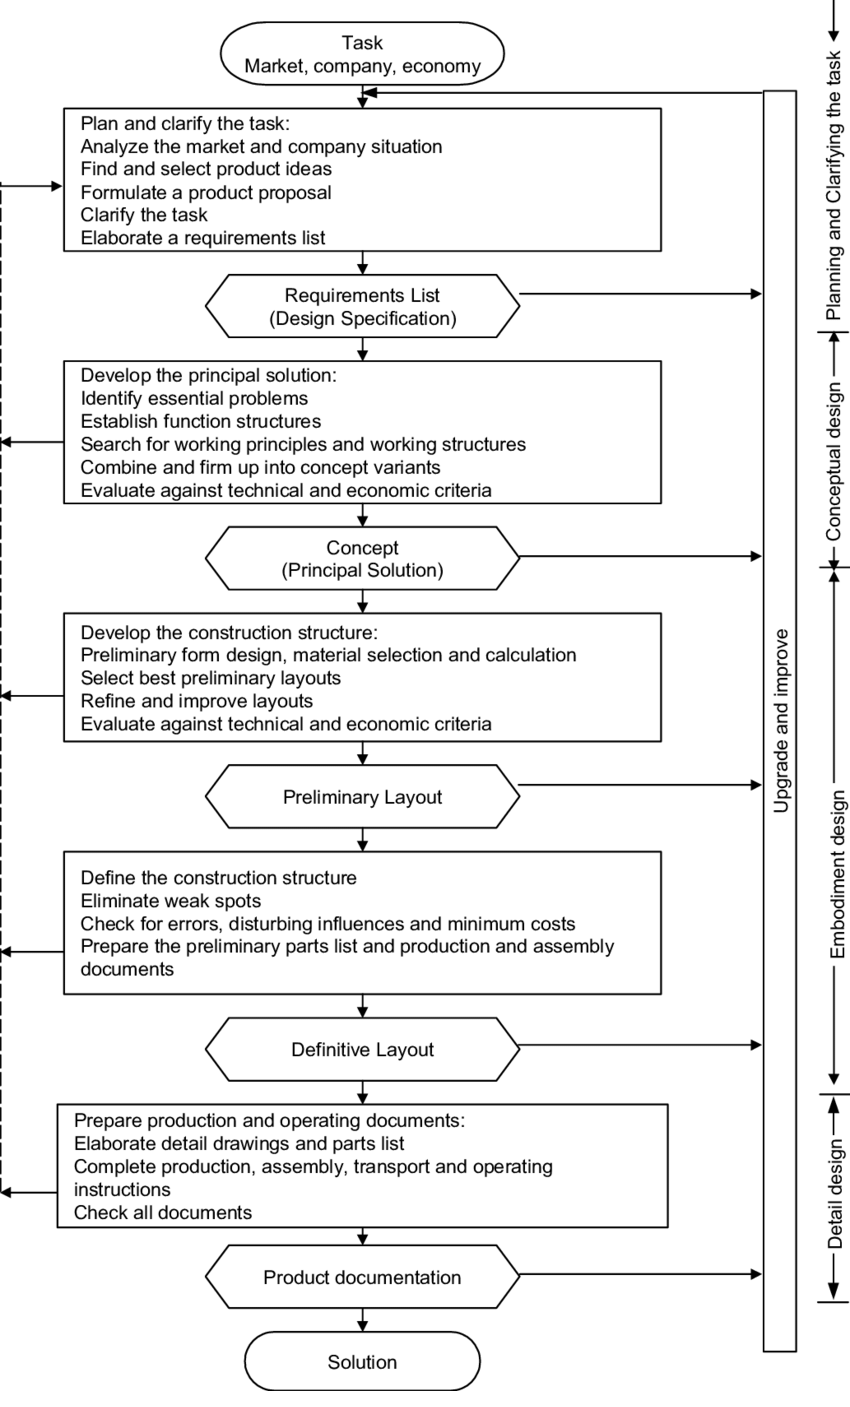
\includegraphics[width=0.8\textwidth]{texs/Part1/chapter1/image/pahlprocess.png}
    \caption{Pahl and Beitz's Design Process \cite{Pahl07l}}
    \label{fig:pahlprocess}
\end{figure}
